\subsection{Extracting the selection efficiency} \label{sec:efficiencyPidExtraction}

Starting from the first selection cut, the CRT-PMT matching, it is possible to see that no difference is present. 
This is explained by the fact that the sample used for this preliminary analysis is composed of only neutrino interactions, i.e., no in-time cosmic interactions are simulated. 
The second cut, Flash-match, has little-to-no effect: this follows from the fact that only one neutrino interaction and no cosmic-ray interaction are present in each event. 
One of the first big differences comes from the request that the vertex has to be located inside the fiducial volume of the detector. 
This is obviously a request that is strongly dependent on the reconstruction performances; therefore, it is expected that an improved reconstruction efficiency, where the vertex reconstruction is improved, would result in such an improvement. 
The following request, that all particles are contained in the active volume of the detector, is also strongly dependent on the reconstruction performances. Correct clustering of the hits and start-/end-point assignation is correlated with a better containment requirement (if the true particles are contained, so should be the reconstructed ones). 
The last selection cuts concern the muon and proton identifications and the no-charged-pion and no-electromagnetic-shower requests. These have a huge impact on the event selection efficiency and, as described before in \autoref{sec:dataSample_and_selection}, are guided not only by the performances of the event reconstruction but also are highly dependent on the TPC calorimetric calibrations (see \autoref{sec:calorimetryAndCalibration}) and on the performances of the particle identification score. This is not only determined by the quality of the topological event reconstruction performed by Pandora, but it is also affected by the calorimetric performances downstream of the Pandora topological event reconstruction. Most of the efficiency loss, namely the ${\sim}\SI{15}{\percent}$ loss in the identification of the proton, followed by the ${\sim}\SI{5}{\percent}$ loss for the identification and rejection of charged pions and electromagnetic showers, is a consequence of the particle identification performed using the calorimetric information.
In the identification of the reconstructed particles there are, however, cuts that do rely on the goodness of the reconstruction, such as the length requirements, the track and shower classification BDT score, the distance from the interaction vertex, and the particle hierarchy requirements. Assuming little correlation between variables that depend on the reconstruction quality and variables that depends on the calorimetric performances, it is possible to factorise their contribution to the final selection efficiency, assigning a ``Pid-related'' event selection efficiency to the latter and a ``reconstruction-related'' event selection efficiency to the former, \begin{equation}
    \epsilon_\mathrm{event\ selection} = \epsilon_\mathrm{ev.\ sel.,\ reco.} \times \epsilon_\mathrm{ev.\ sel.,\ pid}.
\end{equation} 

Getting back to Eq. \eqref{eq:componentsEfficiency}, which can now be written as \begin{equation}
    \begin{aligned}
        \epsilon &= 
        \epsilon_\mathrm{signal\ processing} \times 
        \epsilon_\mathrm{2D\ clusters} \times 
        \epsilon_\mathrm{vertex\ creation} \times 
        \epsilon_\mathrm{3D\ reconstruction} \times \\
        &\quad\quad\quad\times
        \epsilon_\mathrm{particle\ classification} \times 
        \epsilon_\mathrm{event\ selection,\ reco.} \times 
        \epsilon_\mathrm{event\ selection,\ pid}
    \end{aligned} \label{eq:componentsEfficiencyPid}
\end{equation} it is reasonable to postulate a further assumption. 
Since the term $\epsilon_\mathrm{event\ selection,\ reco.}$ is related to the reconstruction efficiency, it is reasonable to assume that this term can be absorbed in terms of the efficiency of each single stage. Supporting this hypothesis is the fact, for example, that once the vertex reconstruction is cheated, the selection request that the vertex is inside the TPC fiducial volume is satisfied, as is possible to deduce from \autoref{fig:efficiencyByCut}. Therefore, Eq. \eqref{eq:componentsEfficiencyPid} can be written as \begin{equation}
    \begin{aligned}
        \epsilon &= 
        \epsilon_\mathrm{signal\ processing} \times 
        \epsilon_\mathrm{2D\ clusters}' \times 
        \epsilon_\mathrm{vertex\ creation}' \times 
        \epsilon_\mathrm{3D\ reconstruction}' \times \\
        &\quad\quad\quad\times
        \epsilon_\mathrm{particle\ classification}' \times 
        % \epsilon_\mathrm{event\ selection,\ reco.} \times 
        \epsilon_\mathrm{ev.\ sel.,\ pid}
        = 
        \epsilon_\mathrm{sig.\ proc.} \times 
        \epsilon_\mathrm{reco.}' \times 
        \epsilon_\mathrm{ev.\ sel.,\ pid},
    \end{aligned} \label{eq:componentsEfficiencyPidNew}
\end{equation} where the prime symbol ($'$) serves the fact that these efficienccies are slightly different from those in Eq. \eqref{eq:componentsEfficiencyPid}. Following the same steps as in Eq. \eqref{eq:componentsEfficiency}-\eqref{eq:stageEfficiencyPrePID} this time it leads to \begin{equation}
    \epsilon_\mathrm{particle\ class.} \times \qty(\frac{
    \epsilon_\mathrm{ev.\ sel., pid}^\mathrm{B}
    }{
    \epsilon_\mathrm{ev.\ sel., pid}^\mathrm{A}
    }) = \frac{
    \epsilon^\mathrm{B}
    }{
    \epsilon^\mathrm{A}
    }. 
\end{equation} For notation ease, the prime is dropped by performing a notation change $\epsilon' \to \epsilon$. At this point, rewriting this equation as \begin{equation}
    \epsilon_\mathrm{particle\ class.} = \frac{
    \epsilon^\mathrm{B}
    }{
    \epsilon^\mathrm{A}
    } \times \frac{
    \epsilon_\mathrm{ev.\ sel., pid}^\mathrm{A}
    }{
    \epsilon_\mathrm{ev.\ sel., pid}^\mathrm{B}
    }, \label{eq:stageEfficiencyPostPID}
\end{equation} it is clear that it is interesting to evaluate the impact of $\epsilon_\mathrm{ev.\ sel.,\ pid}$. To extract such a parameter, the idea was to develop a modified event selection that allowed the effects of particle identification to be decoupled from the effects of the event reconstruction. In this modified event selection, all the cuts performed on variables that depend on the reconstruction performance are left unaltered, whereas the cuts that are dependent on the calorimetric particle identification are ``deceived'' by looking at the true particle labels. The requirements for this ``modified'' particle identification follow.  

\noindent
For the muon in the interaction, the following cuts are applied: \begin{itemize}
    \item the particle should be tagged as a primary particle by Pandora,
    \item the conversion gap should be smaller than \SI{10}{\cm},
    \item the track/shower classification score should be greater than 0.5,
    \item the track length should be greater than \SI{50}{\cm},
    \item the true label should be that of a muon. 
\end{itemize}
For the proton in the interaction, the following cuts are applied: \begin{itemize}
    \item the particle should be tagged as a primary particle by Pandora,
    \item the conversion gap should be smaller than \SI{10}{\cm},
    \item the track/shower classification score should be greater than 0.4,
    \item the reconstructed deposited energy and the true kinetic energy should be greater than \SI{50}{\MeV},
    \item the true label should be that of a proton.
\end{itemize}
For pions, the selection is the same as for protons, with the sole difference of requiring the true label of a charged pion and a lower energy threshold of \SI{25}{\MeV}. 

\noindent
For electromagnetic showers, the following cuts are required: \begin{itemize}
    \item the particle should be tagged as a primary particle by Pandora,
    \item the track/shower classification score should be smaller than 0.5,
    \item the reconstructed deposited energy and the true kinetic energy should be greater than \SI{25}{\MeV},
    \item the true label should be that of an electron of a photon. 
\end{itemize} 

Using this modified event selection, the same selection efficiencies as in \autoref{fig:efficiencyNoNu} are computed. \autoref{fig:CCNp_efficiencyNoNu_cheatingPid} shows the efficiency for the same configurations (see \autoref{tab:configurations}) with the modified event selection. 

\begin{figure}
    \centering
    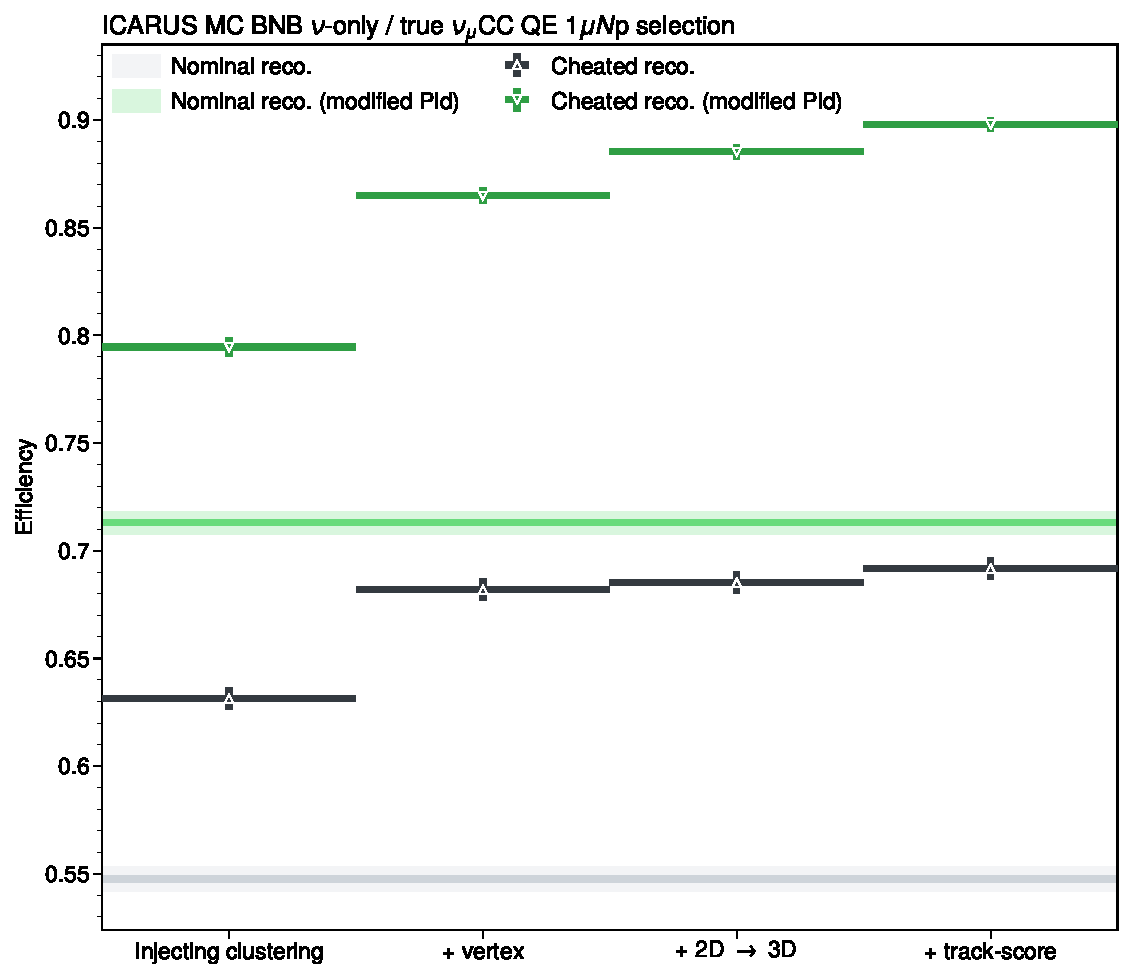
\includegraphics[width=0.85\linewidth]{pandora/chapter_4/CCNp_efficiencyNoNu_cheatingPid.pdf}
    \caption[Evaluation of the reconstruction and selection efficiency for different configurations with the modified event selection]{Evaluation of the event reconstruction and selection efficiency for all the configurations in \autoref{tab:configurations}. Both the event selection with the nominal particle identification (black markers) and the event selection with the modified particle identification (green markers) are shown. }
    \label{fig:CCNp_efficiencyNoNu_cheatingPid}
\end{figure}

% Extracting the efficiency here
For this modified event selection it is possible to assume that the event reconstruction and selection efficiency is \begin{equation}
    \epsilon^\mathrm{mod.\ selection} = \epsilon_\mathrm{sig.\ proc.} \times 
        \epsilon_\mathrm{reco.} \times 
        \epsilon_\mathrm{ev.\ sel.,\ pid}^\mathrm{mod.\ selection}. 
        \label{eq:modifiedPidEfficiency}
\end{equation} It can be assumed that with this modified event selection, the term $\epsilon_\mathrm{ev.\ sel.,\ pid}^\mathrm{mod.\ selection}\simeq1$; therefore, comparing Eq. \eqref{eq:modifiedPidEfficiency} and \eqref{eq:componentsEfficiencyPidNew}, it is possible to extract the efficiency of the particle identification stage for each configuration of \autoref{tab:configurations}. Their ratio leads to \begin{equation}
    \frac{
    \epsilon^{\mathrm{mod.\ selection,}\ c}
    }{
    \epsilon^{c}
    } = \frac{
    \epsilon_\mathrm{sig.\ proc.} \times 
    \epsilon_\mathrm{reco.} \times 
    \epsilon_\mathrm{ev.\ sel.,\ pid}^{\mathrm{mod.\ selection,}\ c}
    }{
    \epsilon_\mathrm{sig.\ proc.} \times 
    \epsilon_\mathrm{reco.} \times 
    \epsilon_\mathrm{ev.\ sel.,\ pid}^c
    } = \frac1{\epsilon_\mathrm{ev.\ sel.,\ pid}^c}
\end{equation} for each configuration $c$. Thereby it is possible to extract \begin{equation}
    \epsilon_\mathrm{ev.\ sel.,\ pid}^c = \frac{
    \epsilon^{c}
    }{
    \epsilon^{\mathrm{mod.\ selection,}\ c}
    }. 
\end{equation} The extracted values of the efficiency of the particle identification stage are reported in \autoref{tab:pidEfficiencyPerConfiguration}. 

\begin{table}[]
    \centering
    \caption[Particle identification efficiency for all configurations]{For each configuration the corresponding efficiency is shown, using both the nominal event selection and the modified event selection described in \autoref{sec:efficiencyPidExtraction}. The third column is the resulting efficiency of the particle identification step. The details are discussed in the text. }
    \label{tab:pidEfficiencyPerConfiguration}
    \begin{tabular}{lp{4cm}ccc}
        \hline
         Id. & Configuration name & $\epsilon$ & $\epsilon^\mathrm{mod.\ selection}$ & $\epsilon_\mathrm{ev.\ sel.,\ pid}$ \\
         \hline
         A & Fully cheated & \SI{69.2(5)}{\percent} & \SI{89.78(33)}{\percent} & \SI{77.1(6)}{\percent} \\
         B & Cheated up to the particle classification algorithm & \SI{68.5(5)}{\percent} & \SI{88.52(35)}{\percent} & \SI{77.4(6)}{\percent} \\
         C & Cheated up to the particle three-dimensional reconstruction algorithm & \SI{68.2(5)}{\percent} & \SI{86.5(4)}{\percent} & \SI{78.8(7)}{\percent} \\
         D & Cheated up to the vertex reconstruction & \SI{63.1(5)}{\percent} & \SI{79.5(4)}{\percent} & \SI{79.4(8)}{\percent} \\
         E & Nominal & \SI{54.8(5)}{\percent} & \SI{71.3(5)}{\percent} & \SI{76.8(9)}{\percent} \\
         \hline
    \end{tabular}
\end{table}

Replacing the corresponding values in Eq. \eqref{eq:stageEfficiencyPostPID} it is possible to get an estimate for the efficiency of each stage of the reconstruction. This leads to the following efficiency values of the reconstruction stages \begin{equation}
    \begin{aligned}
        \epsilon_\mathrm{reco.} =&\
        \epsilon_\mathrm{2D\ clusters} &\times&\ 
        \epsilon_\mathrm{vertex\ creation} &\times&\ 
        \epsilon_\mathrm{3D\ reco.} &\times&\ 
        \epsilon_\mathrm{particle\ class.} =\\  
        =&\ \SI{89.7(1.8)}{\percent} &\times&\ 
        \SI{91.9(1.6)}{\percent} &\times&\ 
        \SI{97.7(1.6)}{\percent} &\times&\ 
        \SI{98.6(1.5)}{\percent}
    \end{aligned}
\end{equation}